% --------------------------------------------------------------
% This is all preamble stuff that you don't have to worry about.
% Head down to where it says "Start here"
% --------------------------------------------------------------
 
\documentclass[12pt]{article}
 
\usepackage[margin=1in]{geometry} 
\usepackage{amsmath,amsthm,amssymb}
\usepackage{algorithmic}
\newcommand{\N}{\mathbb{N}}
\newcommand{\Z}{\mathbb{Z}}
\usepackage{graphicx}
\newenvironment{theorem}[2][Theorem]{\begin{trivlist}
\item[\hskip \labelsep {\bfseries #1}\hskip \labelsep {\bfseries #2.}]}{\end{trivlist}}
\newenvironment{lemma}[2][Lemma]{\begin{trivlist}
\item[\hskip \labelsep {\bfseries #1}\hskip \labelsep {\bfseries #2.}]}{\end{trivlist}}
\newenvironment{exercise}[2][Exercise]{\begin{trivlist}
\item[\hskip \labelsep {\bfseries #1}\hskip \labelsep {\bfseries #2.}]}{\end{trivlist}}
\newenvironment{reflection}[2][Reflection]{\begin{trivlist}
\item[\hskip \labelsep {\bfseries #1}\hskip \labelsep {\bfseries #2.}]}{\end{trivlist}}
\newenvironment{proposition}[2][Proposition]{\begin{trivlist}
\item[\hskip \labelsep {\bfseries #1}\hskip \labelsep {\bfseries #2.}]}{\end{trivlist}}
\newenvironment{corollary}[2][Corollary]{\begin{trivlist}                      
\item[\hskip \labelsep {\bfseries #1}\hskip \labelsep {\bfseries #2.}]}{\end{trivlist}}
\newenvironment{definition}[2][definition]{\begin{trivlist}                      
\item[\hskip \labelsep {\bfseries #1}\hskip \labelsep {\bfseries #2.}]}{\end{trivlist}}
 
\begin{document}
 
% --------------------------------------------------------------
%                         Start here
% --------------------------------------------------------------
 
%\renewcommand{\qedsymbol}{\filledbox}
 
\title{Homework \#2}%replace X with the appropriate number
\author{\\ %replace with your name
CPSC 395 - Analysis of Algorithms
\\ Due: Monday, 28} %if necessary, replace with your course title
\date{}
\maketitle

\begin{enumerate}
\item Exercise 4.1-5 (Use an algorithm package for your algorithm) \\
Use the following ideas to develop a nonrecursive, linear-time algorithm for the maximum-subarray problem. Start at the left end of the array, and progress toward the right, keeping track of the maximum subarray seen so far. Knowing a maximum subarray of A[1..j], extend the answer to find a maximum subarray ending at index j+1 by using the following observation: a maximum subarray of A[1..j+1] is either a maximum subarray of A[1..j] or a subarray A[i..j+1], for some 1 $\leq$ i $\leq$ j+1. Determine a maximum subarray of the form A[i..j+1] in constant time based on knowing a maximum subarray ending at index j.

Linear max subarray algorithm
\begin{algorithmic}
\STATE Find-Max-Subarray-Linear(Array A)
\STATE $alength$ = A.length (Creates variable alength that is equal to length of Array A)
\STATE maxsum = - $\infty$ (This variable will be for the sum for the max subarray found)
\STATE sum = - $\infty$ (This variable is for computing the sum while trying to find the max subarray)
\FOR{j=1 to alength (For loop to iterate through all of the array)} 
\STATE currenthigh= j (This sets the current high to the position of the array that is currently looked at)
\IF{sum $>$ 0} 
\STATE sum = sum + A[j] (If the sum variable is greater than zero, it adds the value of A[j] to the sum)
\ENDIF
\ELSE 
\STATE currentlow = j
\STATE sum = A[j] (This will be the first iteration of the for loop since sum will be less than 0. Set the value of sum to the first value in the array and the low of the current max subarray to j)
\ENDIF
\IF{sum $>$ maxsum (This is when a new max subarray is found and the variables need to be updated)}
\STATE maxsum = sum 
\STATE low = currentlow 
\STATE high = currenthigh (If sum is greater than maxsum, it will update the the low and high of the max subarray and the sum of the array)
\ENDIF
\ENDFOR
\RETURN (low, high, maxsum) (This will return the low and high of the array and the sum of the array)
\end{algorithmic}



\item Exercise 4.4-4 (You can draw the tree by hand, or you can describe the cost at every level of the tree.)\\
Use a recursion tree to determine a good asymptotic upper bound on the recurrence
T(n) = 2T(n-1) + 1. Use the substitution method to verify your answer\\
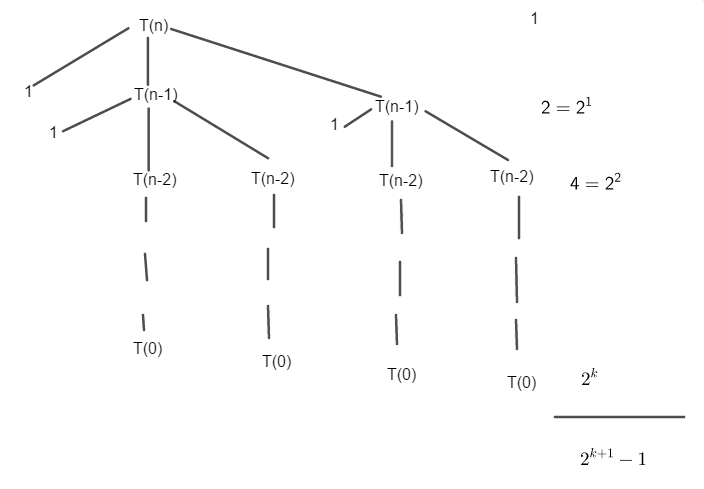
\includegraphics[scale=1]{Recursivetree.png} \\
From the tree we get $2^{n+1} -1$ and we can make a guess of $\Theta$($2^n$). To verify, we will use the substitution method.\\
T(n) = 2T(n-1) + 1 and we can guess that T(n) $\leq$ c$2^n$ + n where c is some constant $>$ 0.\\
T(n) $\leq$ 2 * c$2^{n-1}$ + (n-1) + 1 \\
= $c2^n$ + n \\
= O($2^n$) \\
Therefore, the upper bound is verified and holds true.\\ 

\item Exercise 4.5-1 (give the values of $a,b,c$ and state the case of the theorem you applied)
Use the master method to give tight asymptotic bounds for the following recurrences.\\
\\
T(n) = aT(n/b) + f(n) \\
For the first case, f(n) must be smaller than $n^{log_ba}$. In this case, the solution is T(n) = $\Theta(n^{log_ba})$\\
Second case, if the functions are the same size, we multiply by a log factor and the solution is T(n) = $\Theta(f(n)lgn).$ \\
Third case, the f(n) is larger. The solution is T(n) = $\Theta(f(n))$ \\
\\
a. T(n) = 2T(n/4) + 1 \\ 
a = 2, b = 4, f(n) = 1. In the form of $n^{log_ba}$, $n^{log_42} = n^{1/2}$. F(n) is smaller than $n^{log_ba}$ so this is case 1 and the solution is $\Theta(n^{log_ba})$ = $\Theta(n^{1/2})$ or $\Theta(\sqrt{n})$. \\
\\
b. T(n) = 2T(n/4) + $\sqrt{n}$ \\ 
a = 2, b = 4, f(n) = $\sqrt{n}$.  $n^{log_42}$ = $n^{1/2}$. $n^{1/2}$ can also be written as $\sqrt{n}$ so f(n) and $n^{log_ba}$ are equal. When they are equal, it is case 2 so the solution is $\Theta(n^{log_ba}lgn)$ = $\Theta(n^{1/2}lgn)$ = $\Theta(\sqrt{n}lgn)$\\
\\
c. T(n) = 2T(n/4) + n \\ 
a = 2, b = 4, f(n) = n. $n^{log_42}$ = $n^{1/2}$. F(n) = n is larger than $n^{1/2}$, so we will be using case 3. For case 3, we use $\Theta(f(n))$ so we get $\Theta(n)$\\
\\
d. T(n) = 2T(n/4) + $n^2$ \\
a = 2, b = 4, f(n) = $n^2$. $n^{log_42}$ = $n^{1/2}$ and f(n) is $n^2$. F(n) is larger so we use case 3.  $\Theta(f(n))$ so we get $\Theta(n^2)$.\\

\end{enumerate}
 

% --------------------------------------------------------------
%     You don't have to mess with anything below this line.
% --------------------------------------------------------------
 
\end{document}